 % Die Lösung einiger Security-Probleme, ist eine sichere Datenbank, die die Hashs der versionierten Packete beinhaltet. Bevor man ein Packet installiert können der lokal generierte Hash mit jenem aus der Datenbank verglichen werden, um sicherzustellen, das das Packet das selbe wie bei anderen Usern ist.

 % Um die Datenbank so sicher wie möglich zu gestalten, wird eine Blockchain eingesetzt auf der ein Smart Contract liegt. Dieser smart Contract ermöglicht die Verwendung von Funktionen auf der Blockchain. Mit diesen Funktionen können neue Hashes in die Blockchain geladen werden und es kann der derzeitige Hash eines Paketes und dessen Anzahl abgefragt werden. Hierbei wird garantiert, das von jedem Nutzer für eine Paketversion immer nur ein Hash existiert. Dies ist die erste bekannte Verwendung einer Blockchain für ein solches Problem.

% Der Workflow

% Bild 1 einfügen
% Bild 2 einfügen

% 1) Zuerst wird ein PKGBUILD heruntergeladen und in einer Sandbox teilweise ausgeführt. Die so erhaltenen Daten werden anschließend gehashed.
% 2) Dann wird der Hash mit dem (current consens) Hash des Paketes aus der Blockchain Verglichen (siehe Bild 2). Wenn diese überein stimmen und die Anzahl der commits über dem Threshold liegt wird \texttt{true} zurückgegeben. Ansonsten kann man selbst entscheiden ob man dem lokal generierten Hash vertrauen will oder nicht.
% 3a) Wenn dem Hash vertraut wird kann man sein Paket installieren. Bei dieser Option wird dann der Hash mit der versionierten Packet ID an die Blockchain gesendet und in dieser aufgenommen, insofern dieser User für diese PacketID noch keinen Hash commited hat.
% 3b) Wenn dem Hash nicht komplett vertraut wird, kann man trotzdem das Packet installieren, schickt aber den Hash nicht an die Blockchain.
% 3c) Wenn dem Hash nicht vertraut wird, baut man das Packet anschließend nicht.
% 4) Diese Transaction wird dann an alle Nodes der Blockchain geschickt.
% 5) Sobald eine der Nodes einen neuen Block mined, wird die Transaktion validiert und in der Blockchain verinnerlicht.

% Intro
The solution must therefore be to implement a (preferably distributed) database on the user side, which means that there is no single authoritative source.
Since the aim is to defend against \emph{targeted} attacks, the assumption being that only few users will encounter a malicious version, this can be worked around by checking the hash against a \emph{consensus} formed by many users.

To make the database as safe as possible, a blockchain is used. The chain contains a smart contract providing securely callable functions. With one of these functions it's possible to commit a hash for a package and version. This hash will be saved in the blockchain only if this user has not committed the same hash before, thereby making it harder to take over the blockchain and get a malicious hash to be the consensus. The consensus is updated after every hash commit. Another function is used to get the current consensus hash and its number of commits for a specific package and version.

This appears to be the first project to use a blockchain as a means to provide distributed verification of (software) downloads.

% Workflow
\subsection*{Workflow}
The following workflow is visualized by Figure \ref{fig:main_workflow}.
\begin{figure}
	\centering
		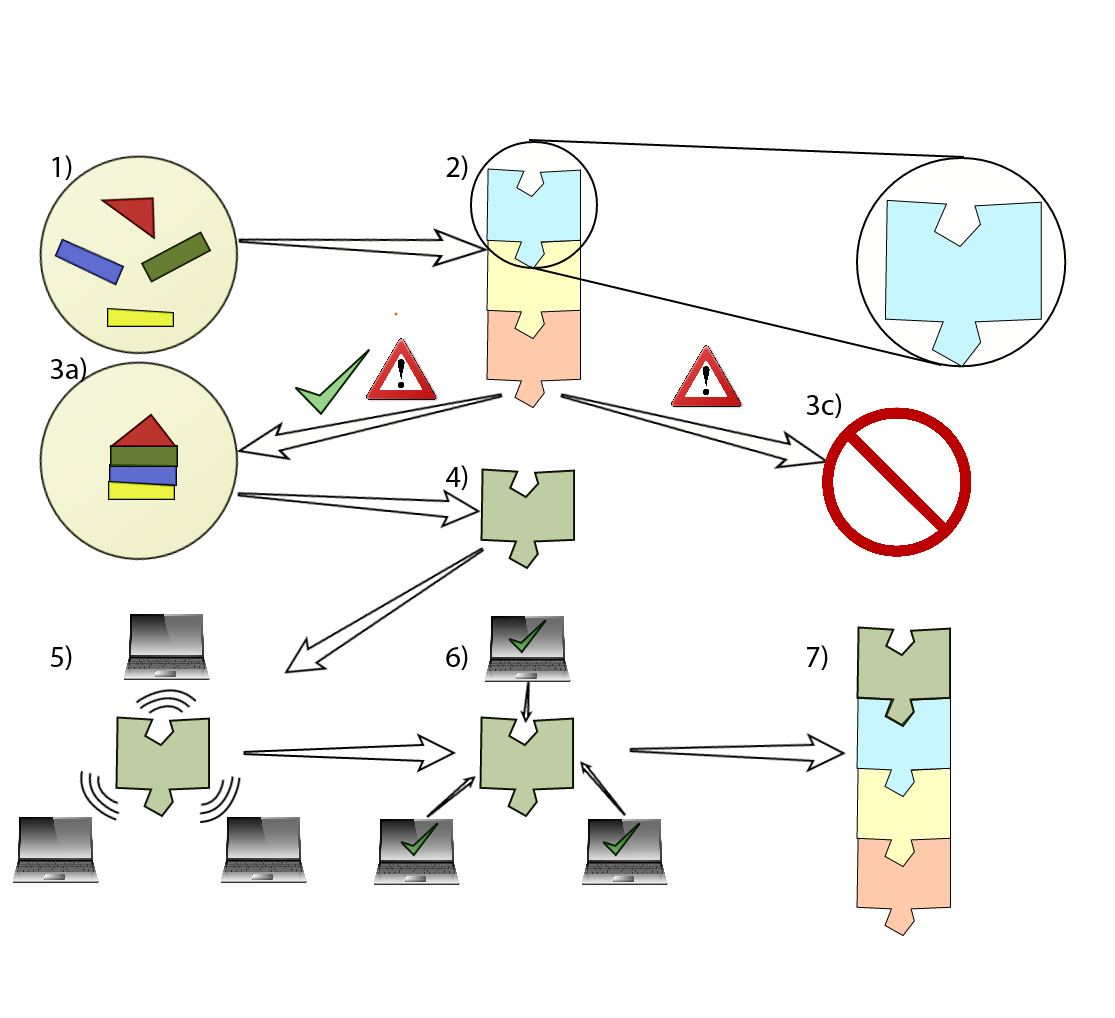
\includegraphics[width=0.6\paperwidth]{Workflow2}
	\caption{Main Workflow}
	\label{fig:main_workflow}
\end{figure}

\begin{figure}
	\centering
		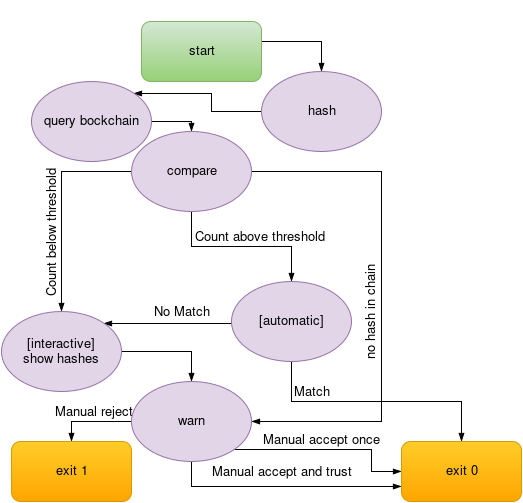
\includegraphics[width=0.45\paperwidth]{workflow}
	\caption{Decision Workflow}
	\label{fig:decision_workflow}
\end{figure}


\begin{enumerate}
	\item First of all a \textit{PKGBUILD} is downloaded and partially executed in a sandbox in order to get the package version. Then, it and any VCS sources are hashed.
	\item The resulting local hash is compared with the current consensus hash on the blockchain. [Figure \ref{fig:decision_workflow}].
	\item Now the workflow splits into 3 different paths:
	\begin{enumerate}
		\item The hashes match and the number of commits is over the threshold or the user decides to trust the locally generated hash anyway. \textit{(Followed by step 4.)} The package may be created and installed.
		\item The hashes don't match and/or the number is below the threshold, but the user want to create and install the package without comitting the hash. \textit{(End of the workflow.)}
		The package may be created and installed.
		\item The hashes don't match and/or the number is below the threshold and the user doesn't want to create the package. \textit{(End of the workflow.)} Our program exits with a non-zero status, so an AUR helper using it would cancel the package installation at this point.
	\end{enumerate}
	\item The local hash is committed to the blockchain (this is a transaction).
	\item All nodes of the blockchain-network get the transaction.
	\item The transaction is contained in the next mined block.
	\item The block is added to the blockchain.
\end{enumerate}
